La seconde partie du processus de \emph{spatialisation} est le
\emph{calcul de la métrique.} C'est durant cette phase qu'est calculée
la mesure utilisée pour quantifier une grandeur que l'on veut
représentative de la sémantique de la \emph{relation de localisation
  atomique} \emph{spatialisée.} Les \emph{métriques} sont plus
nombreuses et diverses que les \emph{rasterisers.}

\subsection{Classification}
Les \emph{métriques} que nous sommes amenés à construire peuvent être
de nature et porter sur des phénomènes assez différents. Toutefois on
peut identifier une certaine récurrence dans leurs
caractéristiques. Tout d'abord, certaines \emph{métriques} quantifient
des phénomènes exprimés par rapport à \emph{l'objet de référence.}
C'est par exemple le cas de la fonction que nous avons précédemment
utilisé pour introduire la méthodologie de \emph{spatialisation.} En
effet, la valeur de cette fonction \footnote{Qui, pour rappel, est de
  1 si la position est confondue avec l'objet de référence et de 0
  sinon.} calculée en un pixel dépend de la position et de la forme de
\emph{l'objet de référence:} si ce dernier change, la \emph{métrique}
change également. Cependant, des \emph{métriques} comme la pente ou
l'altitude, utilisées pour \emph{spatialiser} des \emph{indices de
  localisation} tels que : \enquote{Je suis à \SI{2500}{\meter}} ou
\enquote{Nous sommes dans une zone de forte pente}, ne dépendent pas
d'un \emph{objet de référence.} On parle dans ce cas de
\emph{métriques intrinsèques,} que l'on oppose aux \emph{métriques
  extrinsèques,} telles que la distance à \emph{l'objet de référence}
ou une relation topologique. Un second critère peut être utilisé pour
distinguer les \emph{métriques.}  En effet, certaines d'entre elles
nécessitent un paramétrage pour être calculées. C'est par exemple le
cas d'une \emph{métrique} comme le temps de marche, qu'il est
nécessaire de paramétrer en fonction de la vitesse de
déplacement. Cependant une grande partie des \emph{métriques} ne
nécessitent pas de paramétrage, c'est notamment le cas de la distance
à \emph{l'objet de référence} ou de l'altitude, déjà citées.

Le tableau \ref{fig:type_metriques} catégorise les différentes
\emph{métriques} présentées dans la section suivante en fonction de
ces deux critères.

\begin{table}
  \centering
  \begin{tabular}{>{\bfseries}R{3cm}C{5cm}C{5cm}}
  \toprule
  &
   \multicolumn{1}{c}{\bfseries Paramétriques} &
   \multicolumn{1}{c}{\bfseries Non Paramétriques} \\
  \midrule
  Extrinsèques &&Pente\\
  Intrinsèques &&\\
  \bottomrule
\end{tabular}

  \caption{Types de métriques}
  \label{fig:type_metriques}
\end{table}

\subsection{Les différentes \emph{métriques}}

Parmi tous les exemples que nous avons présentés, une \emph{métrique}
apparait régulièrement : la \emph{distance planimétrique} à
\emph{l'objet de référence.} Le processus de calcul de la
\emph{métrique} consiste à calculer, pour chaque pixel de la \ac{zir},
la distance minimale à \emph{l'objet de référence,} c'est-à-dire la
distance au pixel, appartenant à \emph{l'objet de référence} (défini
lors de la \emph{rasterisation}), le plus proche. Cette métrique a été
utilisée lors de la \emph{spatialisation} de \emph{l'indice de
  localisation} \enquote{Je suis sous une ligne électrique}
(\autoref{fig:ISO_DIST_HT}), mais elle est également utilisable pour
spatialiser des relations topologiques tout en prenant en compte
\emph{l'imprécision} (\eg deux objets très proches, mais qui ne
partagent pas de positions, peuvent, du point vue du requérant, être
considérés comme en contact). Cette \emph{métrique} est un exemple
caractéristique des \emph{métriques extrinsèques} et \emph{non
  paramétriques.} Il est, en effet, nécessaire de la calculer pour
chaque \emph{objet de référence,} mais elle n'accepte pas de
\emph{paramètres.}  On pourrait cependant en ajouter, par exemple en
ajoutant un paramètre permettant d'employer d'autres distances, comme
la distance de Manhattan, de Minkowski ou de Tchebychev. Mais nous
avons estimé que ces distances alternatives, trop éloignées de la
perception humaine des distances, ne présentent pas d’intérêt pour
notre cas d'application.

Une autre \emph{métrique,} également employée lors de la comparaison
des implémentations (\autoref{chap:06}), est la différence d'altitude
entre une position et \emph{l'objet de référence.} Il s'agit d'une
\emph{métrique extrinsèque,} prenant en paramètre la méthode de calcul
du l'altitude de référence, utilisée pour la comparaison. Comme nous
l'avons précédemment (\autoref{tab:atomique_vertical}), plusieurs
méthodes peuvent être employées pour sélectionner l'altitude à
comparer. On peut par exemple calculer la différence d'altitude à
partir de la valeur minimale, maximale ou moyenne de \emph{l'objet de
  référence,} ce qui peut permettre une \emph{spatialisation} plus ou
moins stricte. Cependant, l'usage de ces valeurs de référence n'est
pas pertinent pour des objets très étendus, comme des lignes
électriques ou des forêts. C'est pourquoi nous avons choisi de
calculer par défaut cette différence à partir du pixel de l'objet de
référence le plus proche. Dans cette configuration la \emph{métrique}
\onto{Delta\-Alt} exprime alors une différence d'altitude contextuelle
et non globale comme elle le ferait en calculant la différence par
rapport au maximum ou au minimum. La \autoref{fig:metrique_delta_alt}
donne un exemple ---~extrait de la spatialisation du \emph{fil rouge}
(\autoref{chap:10}) et de la comparaison des implémentations
(\autoref{chap:06})~--- du calcul de cette \emph{métrique.} La
différence d'altitude est ici calculée par rapport à l'altitude du
pixel de la ligne électrique le plus proche. Une amélioration possible
de cette \emph{métrique} serait d'ajouter de nouveaux paramètres
permettant de comparer l'altitude par rapport à des extremums
locaux. Par exemple, en prenant pour point de comparaison le minimum
(ou le maximum ou la moyenne) de la zone la plus proche de
\emph{l'objet de référence.} Cette approche permettrait une plus
grande finesse de \emph{spatialisation,} en permettant des
configurations plus fines. Cependant la solution retenue par défaut à
l'avantage d'être suffisamment robuste pour fonctionner dans toutes
les situations que nous avons rencontrées et ce sans ajustements
\emph{ad hoc.} La métrique \onto{Delta\-Alt} peut également être
utilisée pour calculer une différence par rapport à une altitude
donnée explicitement, comme dans \emph{l'indice de localisation,}
\enquote{Il est à \SI{300}{\meter} d'altitude.}

\begin{figure}
  \centering
  \begin{tikzpicture}
  \tikzset{et/.style={above,font=\footnotesize\vphantom{Ag}}}
  %
  \node[inner sep=0pt, anchor=south west] (image) at (0,0){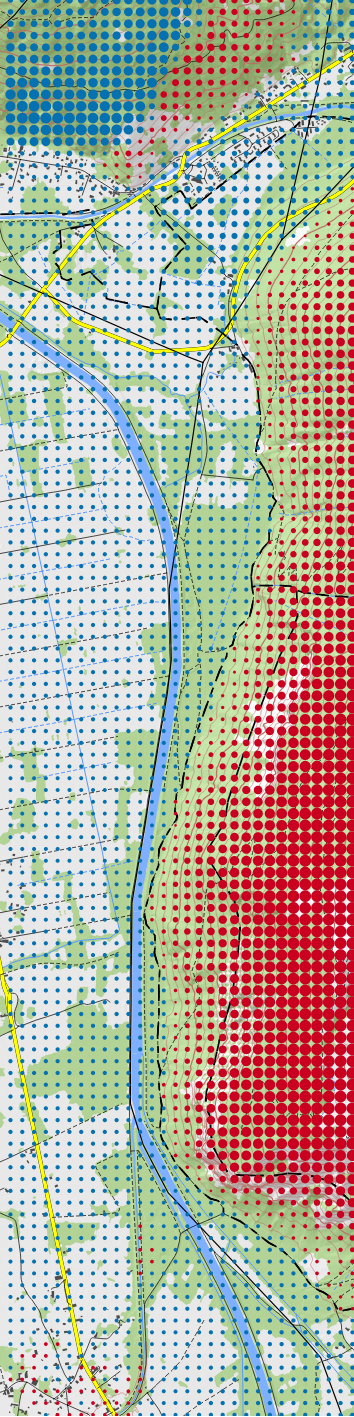
\includegraphics[angle=90]{./figures/Metrique_delta_alt.png}};
  %
  \begin{scope}
    \node (P2) at ([yshift=-.5cm]image.south east) {};
    \node (P1) at ([yshift=-.5cm]image.south west) {};
    %
    \foreach \x [evaluate=\xshift using \x/10, evaluate=\rad using (\x * .0004) + .01] in {0,...,100}
    {
      \draw[fill=black,draw=none, below] ([xshift=\xshift cm, yshift=-.5cm]P1) circle [radius=\rad cm];
    }
    %
    \path(P1 |- 0cm,-1cm) --++ (10,0)
    node[et,pos=0] {0}
    node[et,pos=.1] {0,1}
    node[et,pos=.2] {0,2}
    node[et,pos=.3] {0,3}
    node[et,pos=.4] {0,4}
    node[et,pos=.65] {0,65}
    node[et,pos=1] {1};
    % Échelle
    \draw[-] (P2 |- -1cm,-1cm) --++ (-1,0) node[et,pos=.5] {\SI{500}{\meter}};
    % Légende détaillée
    \path (P1) -- (P2) node[pos=.5, yshift=-1cm] {\tiny Pour la légende détaillée du fond topographique voir \autoref{anx:topo_leg}. Sources: BD TOPO 2018, BD ALTI 2018.}; 
  \end{scope}
\end{tikzpicture}
  \caption{Exemple d'une \emph{métrique} issue de la
    \emph{spatialisation} du \emph{fil rouge,} la différence
    d'altitude par rapport au pixel le plus proche de \emph{l'objet de
      référence.}}
  \label{fig:metrique_delta_alt}
\end{figure}

Pour \emph{spatialiser} les \emph{relations de localisation atomiques}
directionnelles, la \emph{métrique} \onto{Ecart\-Angulaire} a été
développée. Il s'agit d'une \emph{métrique} extrinsèque et
paramétrique. \onto{Ecart\-Angulaire} est destinée à mesurer l'écart à
une orientation donnée, fixée par un paramètre \enquote{angle} et
exprimée à partir de \emph{l'objet de référence.} Cette
\emph{métrique} est employée pour \emph{spatialiser} l'ensemble des
\emph{relations de localisation atomiques} décrivant une orientation
générale, comme les relations de cardinalité (\eg
\onto[orla]{Au\-Nord\-De}). La \autoref{fig:metrique_ecart_angulaire}
donne un exemple de cette \emph{métrique.} À partir d'un point donné
(au centre de la figure) et d'une direction (l'angle supérieur droit),
on construit une demi-droite faisant office de direction de
référence. Puis, pour chaque pixel, on calcule l'écart angulaire
(modulo $2\pi$) entre la direction de référence et la demi-droite
reliant \emph{l'objet de référence} a ce point. Sur la
\autoref{fig:metrique_ecart_angulaire} la valeur absolue de cet angle
est figurée avec une variation de taille, et son signe par une
variation de couleur. Cette \emph{métrique} peut-être utilisée pour
\emph{spatialiser} différentes \emph{relations de localisation
  atomiques.}

\begin{figure}
  \centering
  \begin{tikzpicture}
  \tikzset{et/.style={above,font=\footnotesize\vphantom{Ag}}}
  %
  \node[inner sep=0pt, anchor=south west] (image) at (0,0){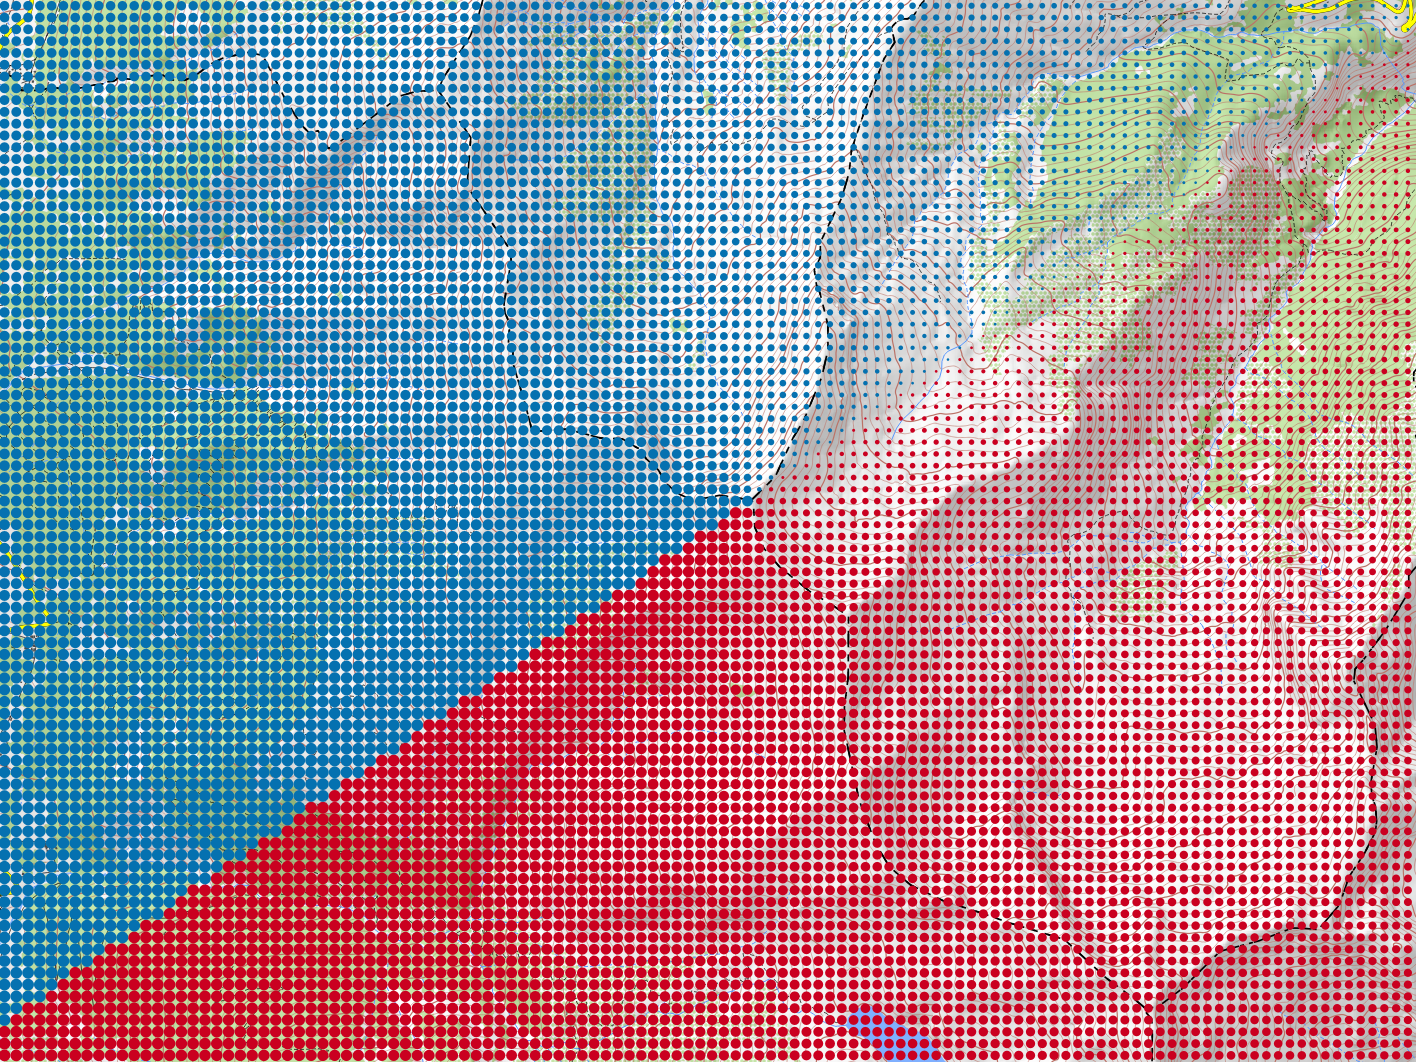
\includegraphics{./figures/Metrique_ecart_valeur.png}};
  %
  \begin{scope}
    \node (P2) at ([yshift=-.5cm]image.south east) {};
    \node (P1) at ([yshift=-.5cm]image.south west) {};
    %
    \foreach \x [evaluate=\xshift using \x/10, evaluate=\rad using (\x * .0004) + .01] in {0,...,100}
    {
      \draw[fill=black,draw=none, below] ([xshift=\xshift cm, yshift=-.5cm]P1) circle [radius=\rad cm];
    }
    %
    \path(P1 |- 0cm,-1cm) --++ (10,0)
    node[et,pos=0] {0}
    node[et,pos=.1] {0,1}
    node[et,pos=.2] {0,2}
    node[et,pos=.3] {0,3}
    node[et,pos=.4] {0,4}
    node[et,pos=.65] {0,65}
    node[et,pos=1] {1};
    % Échelle
    \draw[-] (P2 |- -1cm,-1cm) --++ (-1,0) node[et,pos=.5] {\SI{500}{\meter}};
    % Légende détaillée
    \path (P1) -- (P2) node[pos=.5, yshift=-1cm] {\tiny Pour la légende détaillée du fond topographique voir \autoref{anx:topo_leg}. Sources: BD TOPO 2018, BD ALTI 2018.}; 
  \end{scope}
\end{tikzpicture}
  \caption{Exemple du calcul de la \emph{métrique}
    \protect\onto{Ecart\-Angulaire} pour un point et une direction
    donnée.}
  \label{fig:metrique_ecart_angulaire}
\end{figure}

Bien qu'elle puisse être utilisée à cet effet, la \emph{métrique}
\onto{Ecart\-Angulaire} n'est pas très adaptée à la
\emph{spatialisation} de \emph{relations de localisations} qualifiant
un déplacement vers un \emph{objet de référence,} comme
\onto[orl]{Dans\-La\-Direction\-De}. En effet, un déplacement dans une
direction globale peut conduire à s'éloigner ponctuellement de cette
direction sans que l'on puisse considérer que la \emph{relation de
  localisation spatialisée} soit fausse. Pour prendre en considération
ces cas nous avons développé une \emph{métrique} \emph{ad hoc,}
\onto{Direction\-De}, destinée à quantifier l'éloignement à un
déplacement dans une direction donnée. Le calcul de cette
\emph{métrique} est illustré par la
\autoref{fig:calc_direction_de}. On commence ---~comme pour la
\emph{métrique} \onto{Ecart\-Angulaire}~--- par définir un segment
entre le centre du \emph{l'objet de référence,} le point de départ, et
le centre du second \emph{objet de référence,} la destination. Ce
segment définit la direction de référence, à partir de laquelle la
\emph{métrique} calcule un écart. On ne peut cependant pas calculer
cet écart de la même manière que pour la \emph{métrique}
\onto{Ecart\-Angulaire}, cette mesure ne permettant pas de représenter
des contournements ou des détours qui sont fréquents lors du suivi
d'un itinéraire, d'autant plus dans un milieu montagneux. Nous avons
donc opté pour la définition d'une ellipse, dont la longueur des deux
demi-axes est proportionnel au segment reliant les deux \emph{objets
  de référence.} Cette forme permet de définir une direction
globale. L'écart à cette direction globale peut ensuite être calculé à
l'aide d'une simple distance à l'ellipse. Une illustration de cette
\emph{métrique} est présentée sur la
\autoref{fig:metrique_direction_de}.

\begin{figure}
  \centering
  \begin{tikzpicture}
  \tikzset{et/.style={above,font=\footnotesize\vphantom{Ag}}}
  %
  \node[inner sep=0pt, anchor=south west] (image) at
  (0,0){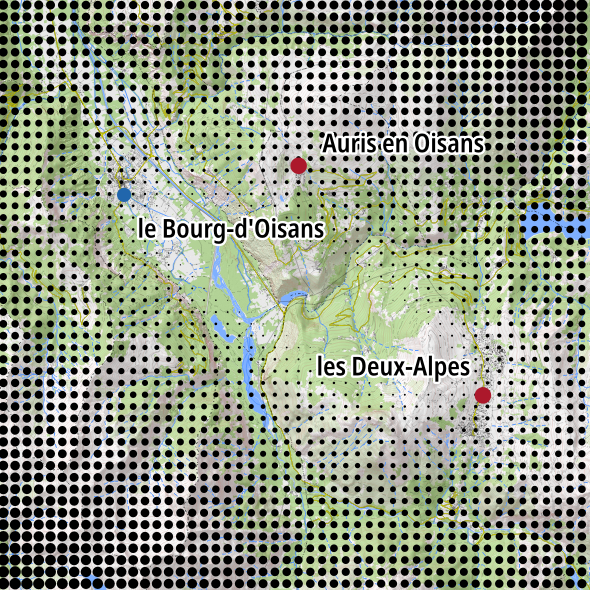
\includegraphics{./figures/EnDirectionDe_metrique_1_FilRouge.png}};
  %
  \begin{scope}
    \node (P2) at ([yshift=-.5cm]image.south east) {};
    \node (P1) at ([yshift=-.5cm]image.south west) {};
    \draw[-] (P2 |- -1cm,-1cm) --++ (-1,0) node[et,pos=.5] {\SI{500}{\meter}}; 
  \end{scope}
\end{tikzpicture}
  \caption{Exemple du calcul de la \emph{métrique}
    \protect\onto{Direction\-De}}
  \label{fig:metrique_direction_de}
\end{figure}

D'autres \emph{métriques,} plus spécifiques (\ie employées par un
petit nombre de \emph{relations de localisation atomiques}) ont
également été développées. C'est par exemple le cas de
\onto{Temps\-De\-Marche} ou \onto{Part\-Visible}, respectivement
utilisées pour la \emph{spatialisation} des \emph{relations de
  localisation} \onto[orla]{Cible\-Voit\-Site} (et son opposée
\onto[orla]{Site\-Voit\-Cible}) et \onto[orla]{A\-Distance\-Temps}
\footnote{Ces trois \emph{relations de localisation atomiques} peuvent
  être utilisées directement. Elles sont par conséquent également
  présentes dans \ac{orl} (\autoref{anx:orl_dic}).}.

La \emph{métrique} \onto{Temps\-De\-Marche} est une \emph{métrique}
extrinsèque, sans paramètre. Sa fonction est de calculer la durée
minimale de déplacement nécessaire pour atteindre chaque pixel de la
\ac{zir} à partir de \emph{l'objet de référence.} Le calcul de cette
\emph{métrique} peut s'effectuer avec un modèle de temps de marche
tels que ceux présentés dans le \autoref{chap:03} (voir
\autoref{fig:modeles_marche}). Ces modèles peuvent calculer, à partir
d'un raster de pente, la durée de traversée d'un pixel. Cette
information est intrinsèque, elle peut donc être pré-calculée et
réutilisée à chaque calcul de la \emph{métrique.} À partir de cette
information et de \emph{l'objet de référence} rasterisé il est ensuite
possible de calculer le temps de parcours minimal de \emph{l'objet de
  référence} à chaque pixel de la \ac{zir}. Dans notre cas nous avons
décidé de calculer la durée de franchissement à l'aide du modèle de
\textcite{Tobler1993} (voir \autoref{eq:marche_tobler}), ce dernier
présentant l'avantage d'être robuste et paramétrable en fonction de la
nature du terrain. On peut ainsi faire évoluer la méthode en modifiant
la durée de franchissement en fonction de la nature du terrain.

Les deux dernières \emph{métriques} que nous avons développées,
\onto{Part\-Visible} et \onto{Part\-Vue}, sont également des
\emph{métriques} extrinsèques et non paramétriques. Elles sont toutes
deux destinées à \emph{spatialiser} des \emph{relations de
  localisations} traitant de visibilité. Ces deux \emph{métriques}
sont très similaires, si ce n'est que la première calcule une zone de
visibilité active à partir de \emph{l'objet de référence} (\ie quels
sont les pixels vus depuis \emph{l'objet de référence}) et la seconde
une visibilité passive (\ie quels sont les pixels qui voient
\emph{l'objet de référence}). La première \emph{métrique} est utilisée
pour \emph{spatialiser} \onto[orla]{Site\-Voit\-Cible} et la seconde
pour \emph{spatialiser} \onto[orla]{Cible\-Voit\-Voit}. La visibilité
est généralement calculée de manière binaire : on vérifie si chaque
pixel de la zone étudiée voit ou non un objet. Le problème d'une telle
\emph{métrique} est qu'elle ne nous permet pas de définir une
visibilité \emph{imprécise,} la zone étudiée est considérée comme
visible ou non. Des pistes pour une modélisation \emph{imprécise} de
la visibilité ont été proposées par
\textcite{Fisher1991,Fisher1992}. Une des solutions proposées étant
d'étudier la variation des zones de visibilité en fonction des
modifications du \ac{mnt} de référence, pour identifier les zones où
la visibilité est la plus variable et donc potentiellement la plus
\emph{imprécise.}  Nous avons cependant opté pour une autre approche,
considérant que \emph{l'imprécision} de la visibilité doit quantifier
la qualité de la perception de \emph{l'objet de référence} que la
qualité des données servant a son calcul. Nous avons donc construit
des \emph{métriques} calculant la part visible de \emph{l'objet de
  référence.} Ainsi, pour chaque pixel de la \ac{zir} nous calculons,
non pas si \emph{l'objet de référence} est visible, mais quelle est la
part de ses pixels qui le sont. On obtient alors un raster dont les
valeurs varient de 0, lorsque l'objet n'est pas visible, à 1 lorsque
tous les pixels qui le représentent le sont. On peut voir une
illustration du calcul de la \emph{métrique} \onto{Part\-visible} sur
la \autoref{fig:metrique_part_lac}. Dans cet exemple la taille du
figuré représente la part de \emph{l'objet de référence} (le lac au
centre de l'image) qui est visible depuis chaque pixel.

\begin{figure}
  \centering
  \begin{tikzpicture}
  \tikzset{et/.style={above,font=\footnotesize\vphantom{Ag}}}
  %
  \node[inner sep=0pt, anchor=south west] (image) at (0,0){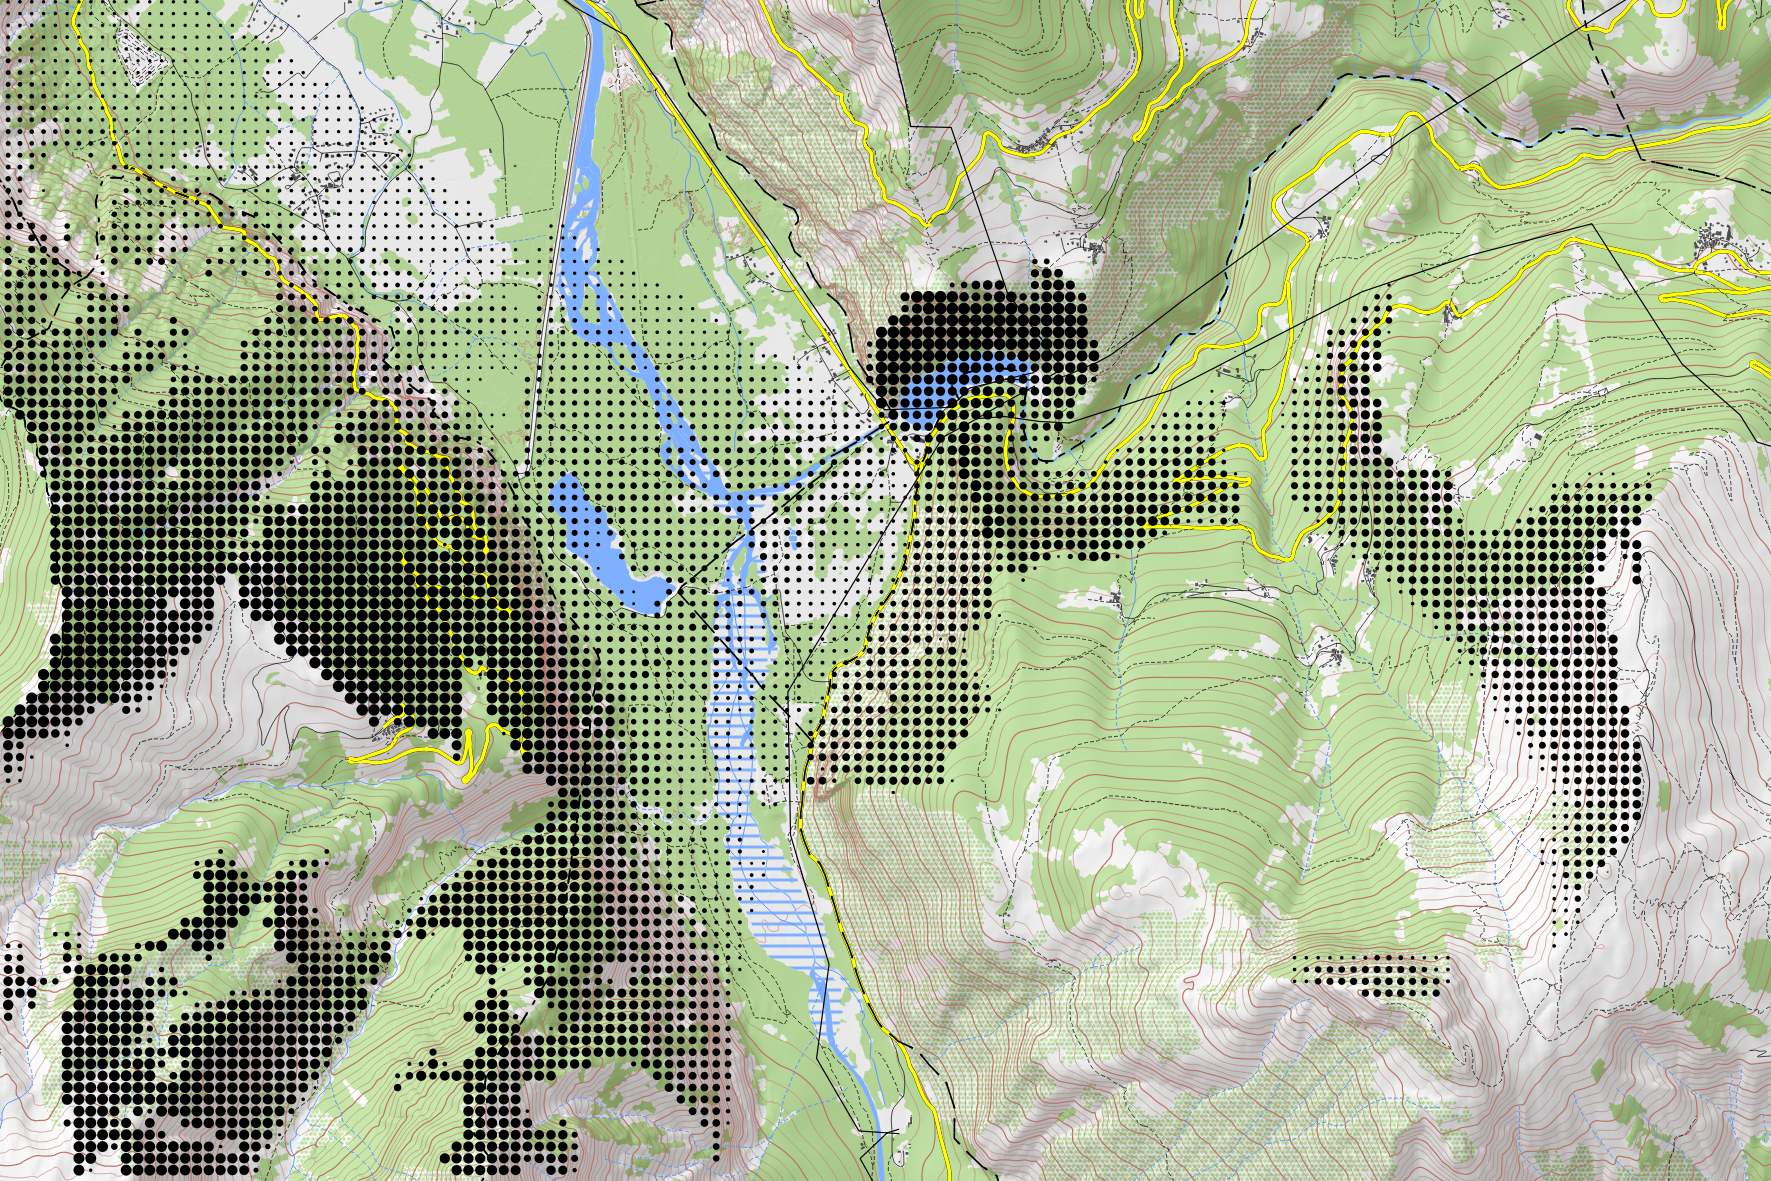
\includegraphics{./figures/Metrique_part_lac_visible.png}};
  %
  \begin{scope}
    \node (P2) at ([yshift=-.5cm]image.south east) {};
    \node (P1) at ([yshift=-.5cm]image.south west) {};
    %
    \foreach \x [evaluate=\xshift using \x/10, evaluate=\rad using (\x * .0004) + .01] in {0,...,100}
    {
      \draw[fill=black,draw=none, below] ([xshift=\xshift cm, yshift=-.5cm]P1) circle [radius=\rad cm];
    }
    %
    \path(P1 |- 0cm,-1cm) --++ (10,0)
    node[et,pos=0] {0}
    node[et,pos=.1] {0,1}
    node[et,pos=.2] {0,2}
    node[et,pos=.3] {0,3}
    node[et,pos=.4] {0,4}
    node[et,pos=.65] {0,65}
    node[et,pos=1] {1};
    % Échelle
    \draw[-] (P2 |- -1cm,-1cm) --++ (-1,0) node[et,pos=.5] {\SI{500}{\meter}};
    % Légende détaillée
    \path (P1) -- (P2) node[pos=.5, yshift=-1cm] {\tiny Pour la légende détaillée du fond topographique voir \autoref{anx:topo_leg}. Sources: BD TOPO 2018, BD ALTI 2018.}; 
  \end{scope}
\end{tikzpicture}
  \caption{Exemple d'une \emph{métrique} issue de la
    \emph{spatialisation} du \emph{fil rouge :} la part de la surface
    visible d'un lac donné.}
  \label{fig:metrique_part_lac}
\end{figure}

%%% Local Variables:
%%% mode: latex
%%% TeX-master: "../../../../main"
%%% End:
